% $Id: assembly.tex 9373 2021-08-30 21:03:39Z mskala $

%
% MSK 012 build instructions
% Copyright (C) 2018, 2019, 2020, 2021  Matthew Skala
%
% This program is free software: you can redistribute it and/or modify
% it under the terms of the GNU General Public License as published by
% the Free Software Foundation, version 3.
%
% This program is distributed in the hope that it will be useful,
% but WITHOUT ANY WARRANTY; without even the implied warranty of
% MERCHANTABILITY or FITNESS FOR A PARTICULAR PURPOSE.  See the
% GNU General Public License for more details.
%
% You should have received a copy of the GNU General Public License
% along with this program.  If not, see <http://www.gnu.org/licenses/>.
%
% Matthew Skala
% https://northcoastsynthesis.com/
% mskala@northcoastsynthesis.com
%

\chapter{Building the module}

In order to achieve 6HP width, this module is built with a couple of
components (the switch and LED) mounted off the board and connected by
``flying'' hookup wires.  The board is crowded, especially where
the wires attach, so it is recommended to install the
components in the order described here:  first the small on-board
components, then the wired-in panel components, then the larger on-board
components, and finally the rest of the panel components.  If you leave the
wired components until too late, it can be difficult to fit the wires into
the board.

Although I'm describing a separate step for each component value, and that's
how I built mine so as to have plenty of photo opportunities, if you are
reasonably confident about your skills you may find it easier to put most
components in place first and then solder them in a single step.  Except for
the overall sequence of putting in the wires before the board gets too
crowded, the order does not matter much.

The board shown in my photos here is a version 3 board, which is
the version shipped in North Coast kits; but some earlier boards
were used in prototypes and early runs of pre-assembled modules.  If you
disassemble a pre-assembled module, there may be minor
differences in the silkscreen, in particular showing component values that
were changed in development.

\section{Preliminaries}

Count out the right number of everything according to the bill of materials
on page~\pageref{cha:bom}. 

{\nopagebreak
\noindent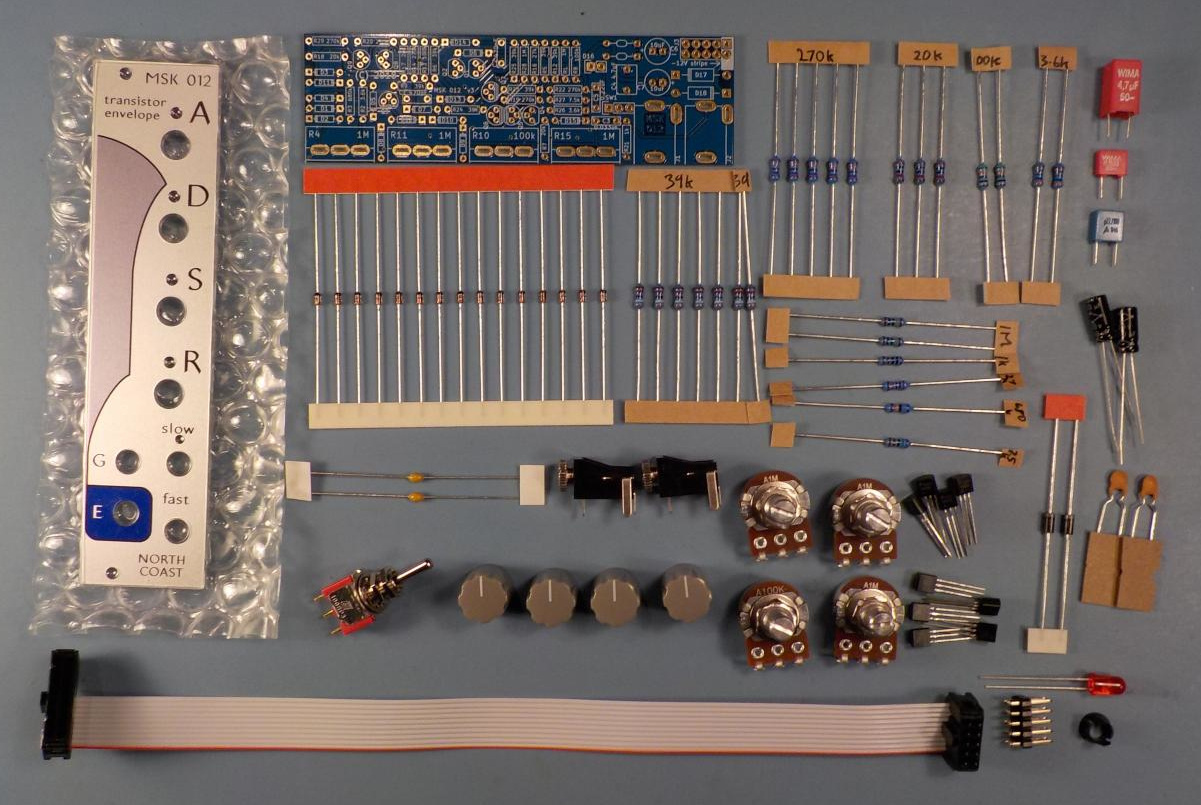
\includegraphics[width=\linewidth]{board-parts.jpg}}

\section{Some notes on knobs}

The first batch of knobs I ordered for North Coast products turned out to
have serious quality problems, specifically with the setscrews that hold the
knobs onto the potentiometer shafts.  Some of the screws had marginal
threads that would strip when the screw was tightened, and I ended up having
to do a bunch of extra testing and ship extra knobs to some customers to
replace any that might fail.  Later batches have also had issues, although
they're under better control now because the bad first batch served as a
warning to step up the testing procedures.  Starting with kits prepared in
August 2019, I switched to blue knobs with 100\%\ testing; in September
2020, I switched to a new manufacturer, and knobs that are a slightly darker
shade of blue.  Although all the knobs I ship in kits now have been tested
and passed at least twice, and should be fine to use, I am also shipping
spare setscrews in any kits with knobs from batches where a signficant
number of knobs failed testing.

Here are some things to be aware of as a kit builder.

\begin{itemize}
\item Some photos in these instructions were taken with the older grey
knobs, and some dealers may still have kits containing grey knobs in their
stock, but newer kits will have blue knobs.

\item Do not overtighten the setscrews when attaching the knobs!  The screw
should be tight enough to hold the knob onto the shaft, but there's no
advantage to making it tighter than that, and overtightening may risk
destroying the screw thread or damaging the drive slot.

\item If, despite my efforts to make sure no bad screws get sent to
customers, you still get a bad screw that cannot be tightened and no spare
for it, then please contact me.

\item If you want to source an exact replacement for the setscrew, it should
be an M3$\times$3mm flat-tip slotted setscrew, which is also sometimes
called a ``grub screw,'' made of RoHS-compliant brass (possibly by
exemption).  Stainless steel is fine too, and I may sometimes ship stainless
steel screws instead of brass if I can find a reliable source for them;
plain steel should not be used here for galvanic corrosion reasons. 
Hex-socket screws are fine if you have the driver for them, but I don't ship
those because I'm not sure all DIY builders do have the right driver.

\item Because it's a standard M3 thread, in a pinch it's possible to
substitute a plain M3 machine screw such as are commonly used with Eurorack
cases, although one of those would obviously look less nice.
\end{itemize}

\section{Diodes}

Install the two Schottky diodes D17 and D18.  These protect the module against
reverse connection of the power supply.  They are polarized and must be
installed in the correct direction; otherwise they will prevent the module
from operating.  One end of each diode will be marked, usually with a stripe
of grey paint around the black plastic body of the diode.  That end is the
\emph{cathode}.  The diode outline on the PCB silkscreen is marked with a
similar stripe showing the direction of the cathode, and the solder pad for
the cathode is square instead of round.

\noindent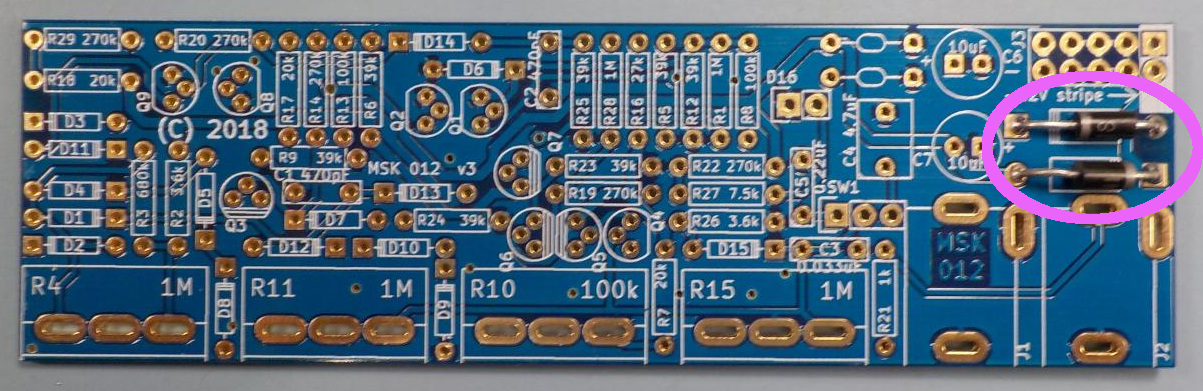
\includegraphics[width=\linewidth]{schottky.jpg}

Install the 15 1N4148 or 1N914 switching diodes D1 to D15.  These switch
currents around, and provide controlled voltage drops, to sequence the
different stages of the envelope.  As with the Schottky diodes, these are
polarized, with the cathode indicated by a stripe on the diode body (usually
a black stripe on the orange-pink glass) and a stripe and square pad on the
PCB.

\nopagebreak
\noindent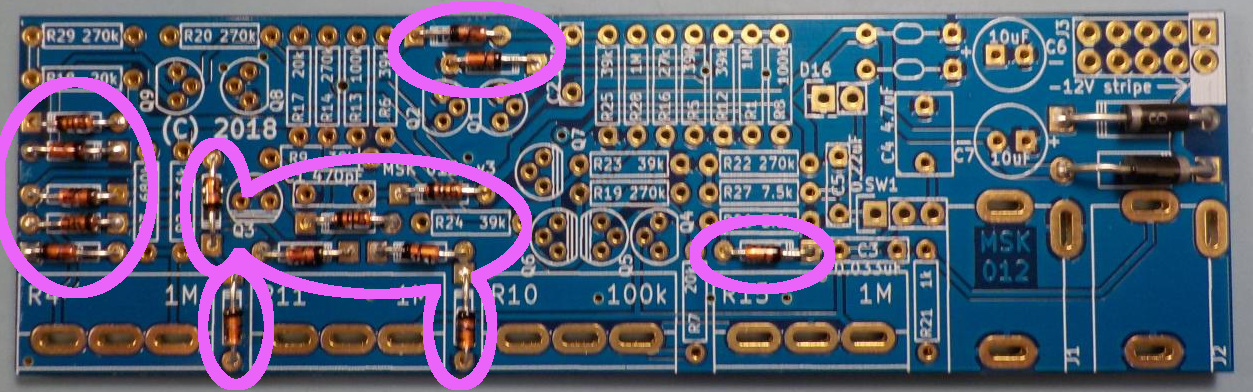
\includegraphics[width=\linewidth]{1n4148.jpg}

\pagebreak

\section{Decoupling capacitors}

The two axial ceramic 0.1$\mu$F decoupling capacitors are shown on the board
by a special symbol without their reference designators.

\noindent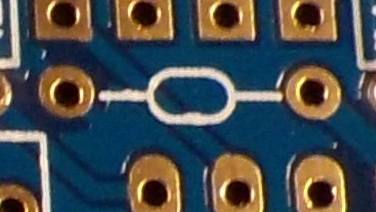
\includegraphics[width=\linewidth]{decoup-symbol.jpg}%
\label{pag:decoup-symbol}

Install these capacitors where the symbol appears.  They are not polarized
and may be installed in either orientation.  They act as filters for
high-frequency noise on the power busses.

\noindent\includegraphics[width=\linewidth]{{cap-0.1u}.jpg}

\section{Fixed resistors}

Resistors are never polarized.  I like to install mine in a consistent
direction for cosmetic reasons, but this is electrically unnecessary.  In
this module, metal film 1\%\ resistors are recommended for all fixed-value
resistors.  These will usually have blue bodies and four colour bands
designating the value, plus a fifth band for the tolerance, brown in the
case of 1\%.  These are the resistors normally shipped in the
North Coast kits, but we may occasionally ship better-tolerance resistors (such
as 0.5\%) if we are able to source them at a good price. 
Accordingly, I mention only the four value band colours for this type of
resistor; if you are using resistors with other codes, you are responsible
for knowing them.  Note that colour codes on metal film 1\% resistors are
often ambiguous (reading from one end or the other end may give two
different values, both plausible) and some of the colours are hard to
distinguish anyway.  If in doubt, always measure with an ohmmeter before
soldering the resistor in place.

Install the 1.0k$\Omega$ (brown-black-black-brown) resistor R21.  This is a
current-limiting resistor for the envelope output, to protect both the
MSK~012 and the external circuit in case the output is connected to an
excessively low impedance.

\noindent\includegraphics[width=\linewidth]{{res-1.0k}.jpg}

Install the two 3.6k$\Omega$ (orange-blue-black-brown) resistors R2 and R26. 
The resistor R2 limits the maximum current into the capacitor during attack,
and the resistor R26 is the emitter resistor (which sets overall
power level) for the output driver.

\noindent\includegraphics[width=\linewidth]{{res-3.6k}.jpg}

Install the 7.5k$\Omega$ (violet-green-black-brown) resistor R27.  This sets
the current through, and therefore the brightness of, the LED.

\noindent\includegraphics[width=\linewidth]{{res-7.5k}.jpg}

Install the three 20k$\Omega$ (red-black-black-red) resistors R7, R17, and
R18.  The first of these, R7, sets the high end of the adjustment range for
sustain voltage; R17 and R18 are collector resistors, controlling the
current drawn in the ``on'' and ``off'' states, for the transistors in the
attack flip-flop.

\noindent\includegraphics[width=\linewidth]{{res-20k}.jpg}

\pagebreak

Install the 27k$\Omega$ (red-violet-black-red) resistor R16.  Do not confuse
this one with the five 270k$\Omega$ resistors to come later, which have
orange bands in the fourth colour code position.  This resistor controls the
trigger level for the output Schmitt trigger, and thus the peak voltage
attained during the attack phase.

\noindent\includegraphics[width=\linewidth]{{res-27k}.jpg}

Install the seven 39k$\Omega$ (orange-white-black-red) resistors R5, R6, R9,
R12, R23, R24, and R25.  Four of these (R5, R6, R23, and R24) are collector
resistors for the transistors in the input and output Schmitt triggers.  Two
(R9 and R25) control the pulse length for the pulse outputs of those Schmitt
triggers.  The remaining one (R12) controls the sensitivity of the gate
input.

\noindent\includegraphics[width=\linewidth]{{res-39k}.jpg}

Install the two 100k$\Omega$ resistors (brown-black-black-orange; photo
shows 0.5\% resistors with green tolerance bands) R8 and R13.  The first
sets the module's input impedance and the second provides current to the
sustain-level potentiometer.

\noindent\includegraphics[width=\linewidth]{{res-100k}.jpg}

\pagebreak
Install the five 270k$\Omega$ (red-violet-black-orange) resistors R14, R19,
R20, R22, and R29.  These are used in multiple locations throughout the
module to provide weak default voltage or current levels, which will be
overridden by stronger signals at the appropriate points in the envelope
cycle.

\noindent\includegraphics[width=\linewidth]{{res-270k}.jpg}

Install the 680k$\Omega$ (blue-grey-black-orange) resistor R3.  This sets
the overall range of the attack speed.

\noindent\includegraphics[width=\linewidth]{{res-680k}.jpg}

Install the two 1.0M$\Omega$ (brown-black-black-yellow) resistors R1 and
R28.  These act as weak positive feedback paths in the Schmitt triggers,
creating the hysteretic effect that defines such circuits.

\noindent\includegraphics[width=\linewidth]{{res-1.0m}.jpg}

\section{Wired panel components}

First, some notes on wire.  You will need five pieces of hookup wire, each
about 3 inches (7.5 centimetres) long, preferably in at least three colours. 
North Coast kits are specified to come with three pieces each 6 inches long,
in three different colours; cut each in half and you will have the requisite
five pieces plus one spare.  Do not use wires much longer or shorter than
specified or you may find that either they will not reach from the board to
the panel properly, or you have a tangled mess of excess wire which will not
fit in the space the module must occupy.  The wires in a kit should be in
three different colours but not necessarily exactly the colours shown in the
photos here.

We recommend (and ship in the kits) pre-tinned stranded copper wire.  If you
use plain copper, you will need to tin it, and to do so carefully so as not
to make the overall wire diameter too thick to fit through the holes on the
PCB.  Stranded wire should not be soldered with water-soluble (often
misleadingly called ``organic'') flux because it is not realistically
possible to remove all traces of it from between the strands.  However,
using some added non-water-soluble flux from a flux pen on these connections
is a good idea to help make the connections with as little excess heat as
possible, especially on the LED, which is heat-sensitive.

Prepare five pieces of hookup wire, each 3$''$ (7.5cm) long.  Strip the
ends, and tin them if necessary.

\noindent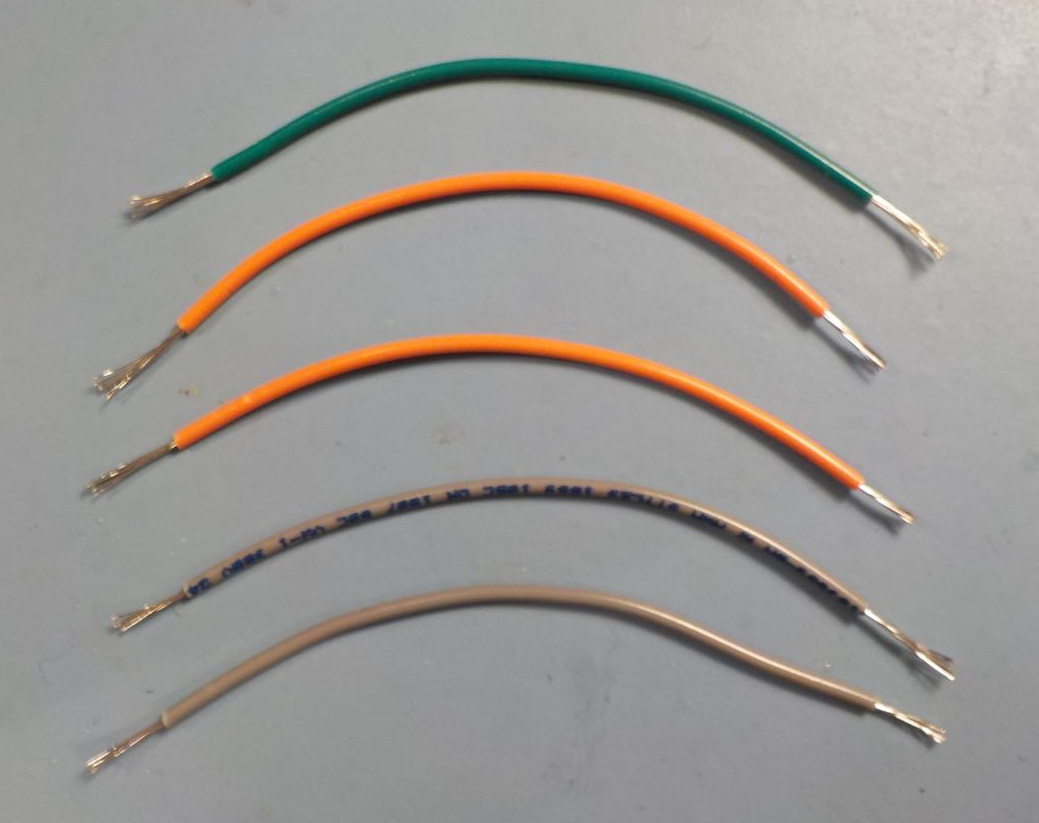
\includegraphics[width=\linewidth]{wires.jpg}

The LED, D16, is a polarized component.  One of its two legs is the cathode,
identified by a shorter leg, a flattened side on the plastic package, and a
much larger metal terminal visible inside the plastic.  Since the cathode
will connect to the 0V plane, I suggest using a black, grey, or darker
coloured wire for it.

\pagebreak

Cut the LED legs to about $\tfrac{1}{2}''$ (13mm) length.  Form them into
hooks, trying to place as little stress on the place the wires enter the
LED's plastic body as possible.  Take two pieces of hookup wire, form one
end of each into a hook, and link them with the hooked legs of the LED.  Be
sure you know which colour you have used for the cathode (grey is shown in
the photo).  Then pinch the hooks closed to form a mechanical connection.

\nopagebreak
\noindent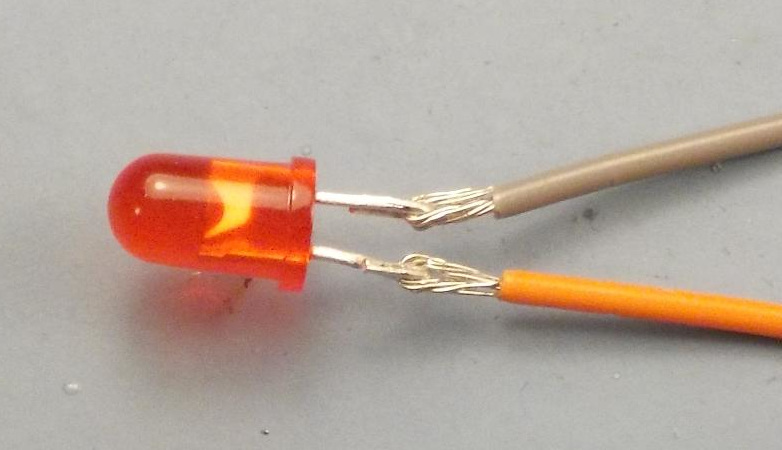
\includegraphics[width=\linewidth]{led-mechanical.jpg}

Carefully solder the LED connections, using as little excess heat as
possible.  If you are concerned about this point, you might use a clip-on
heat sink on the LED legs to reduce the amount of heat conducted into the
LED body.  Dabbing the connections with a non-water-soluble flux pen before
soldering may also be a good idea.  After soldering, if your flux was not a
no-clean type, you should remove the flux with solvent; it should be safe to
dip the entire LED assembly at this point into any reasonable flux-cleaning
solvent.

Take the remaining three pieces of hookup wire and form one end of each into
a hook.  Hook them through the holes on the terminals on the SPDT toggle
switch SW1, then pinch them closed to form mechanical connections.  There is
no specific colour code recommended, but it is recommended to use three
different colours for the three terminals because their arrangement is
significant.

\noindent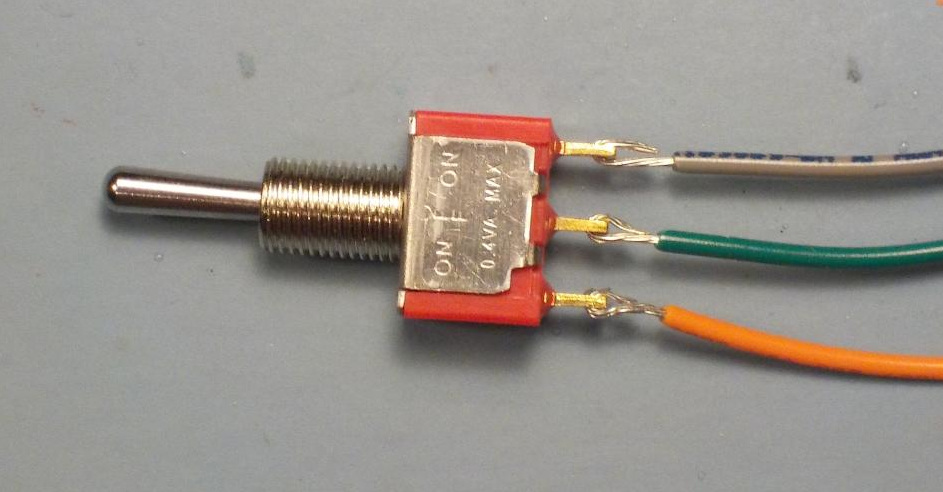
\includegraphics[width=\linewidth]{switch-mechanical.jpg}

Solder the three switch terminals.  The switch is less heat-sensitive than
the LED, but some added no-clean flux is still recommended.  The switch
cannot safely be dipped in solvent, so if you need to clean these
connections after soldering, you will need to use a brush.

Cut five small pieces of heat-shrink tubing and place them over the
connections on the LED and switch.  North Coast kits come with significantly
more heat-shrink tubing than is required here and you should have some left
over; do not attempt to use it all or you will make the wires too stiff to
be bent into the space they must occupy.

\noindent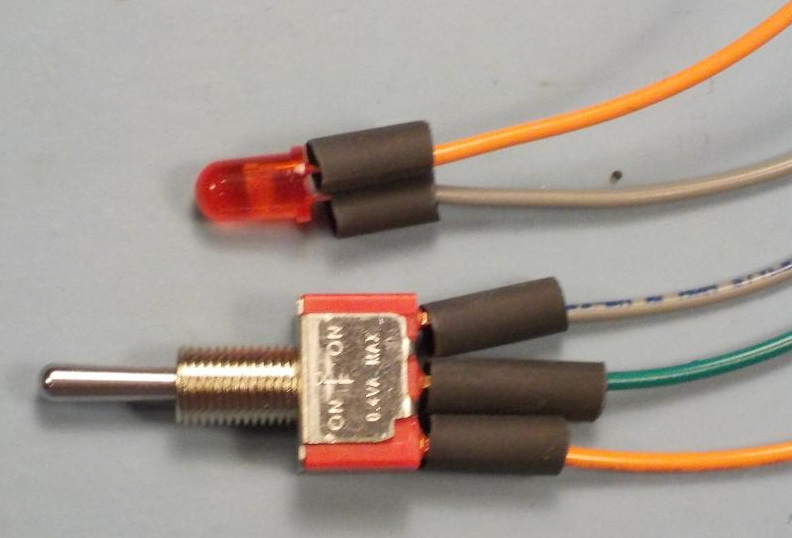
\includegraphics[width=\linewidth]{heat-shrink.jpg}

Carefully shrink the heat-shrink tubing.  The best way to do this is with a
hot-air gun made specifically for electronics assembly, on a relatively low
temperature setting (cooler than would be appropriate for hot-air
soldering).  The stream of hot gasses above a candle flame will work, with a
fair bit of caution.  A hair dryer may possibly work.  Heat from both sides
to shrink the tubing evenly around the solder joints.

Do not have containers of, or brushes or rags contaminated with, flux
cleaner or similar products open nearby while working with any open flame. 
Do not overheat the heat-shrink tubing so that it melts completely, chars,
or catches fire; do not overheat other plastic parts so that they melt. 
After shrinking, the heat-shrink tubing will be very soft and fragile until
it fully cools; do not touch it until then.

Put the free ends of the hookup wires into the holes for the D16 and SW1
footprints on the PCB.  The cathode of D16 (as described above) should
connect to pin 1 of the D16 footprint, denoted by a square pad and further
away from the end of the board where the power header and Schottky diodes
are.  The switch has a groove or keyway on its bushing, to mate with a tab
on the anti-rotation ring.  The terminal nearest that groove should connect
to pin 1 of the SW1 footprint, again denoted by a square solder pad and
furthest away from the power end of the board, with the other two terminals
in sequence from there.  Twisting the wires together for a neater appearance
is optional.

\noindent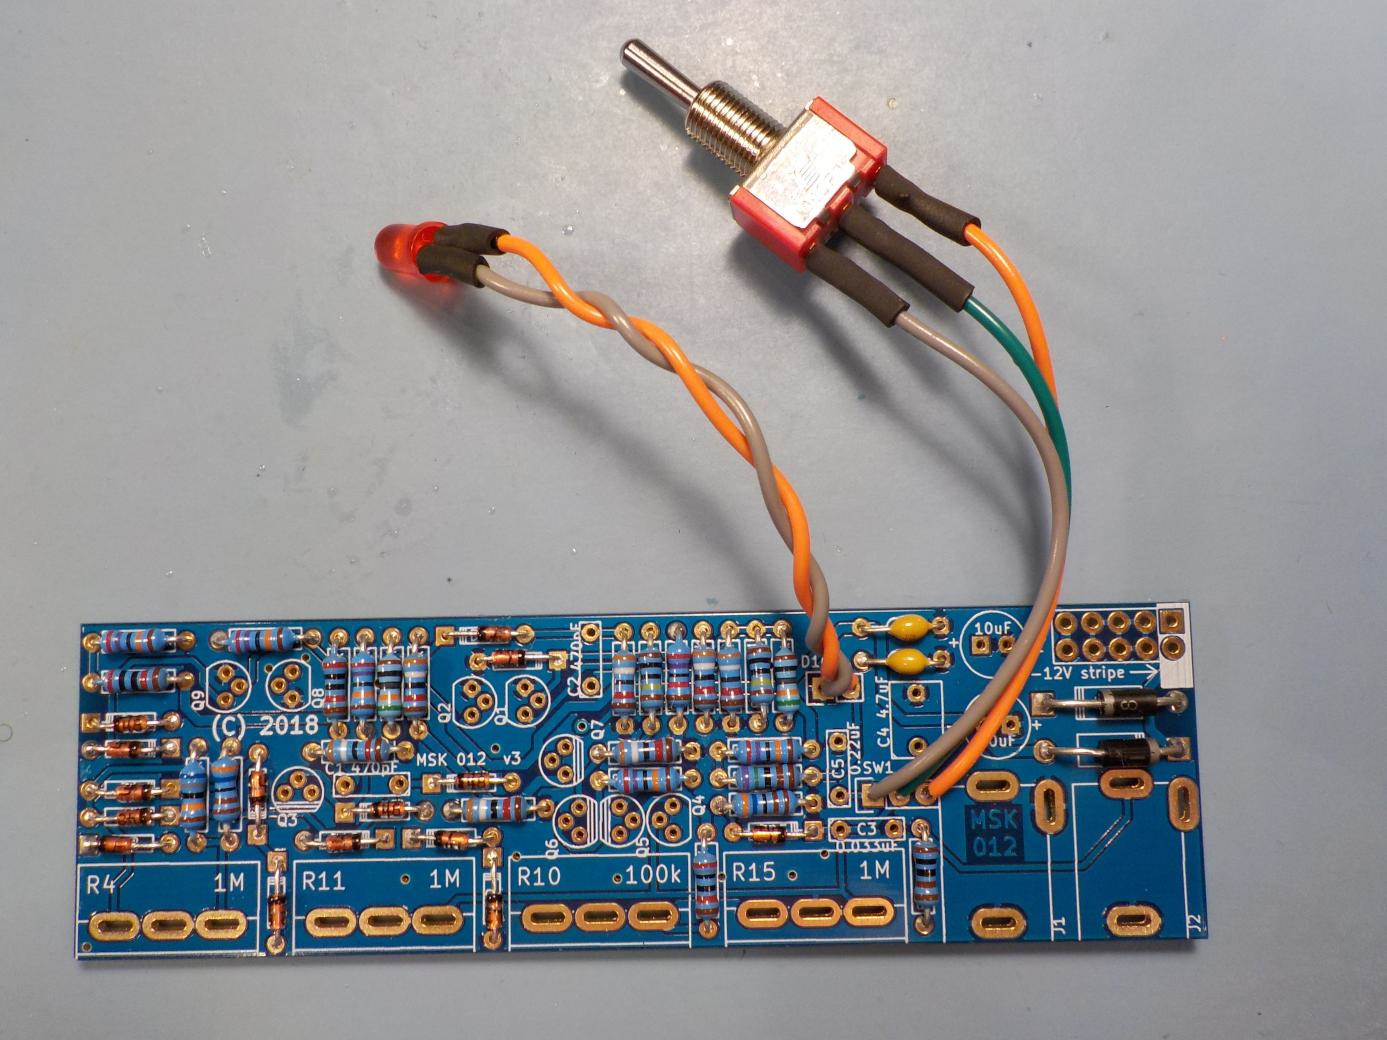
\includegraphics[width=\linewidth]{wires-to-board.jpg}

Solder the wires to the board.

\section{Transistors}

The MSK~012 contains two different types of transistors packaged in TO-92
packages.  Each looks like a little black pill of epoxy plastic with one
flat side and three metal legs; they can be distinguished by etched or
printed numbers on the flat side, and it is important to sort them carefully
and install only the proper component type in each footprint.

There is not enough space on the boards to print a part number for every
TO-92 component, but there are two different silkscreen symbols used to help
with recognition.  The SS8550D or PN200A transistors are shown on the board
with extra silkscreen lines along the flat edge, as in the left photo.  The
2N5088 transistors are shown by a plain outline without extra lines, as in
the right photo.

\noindent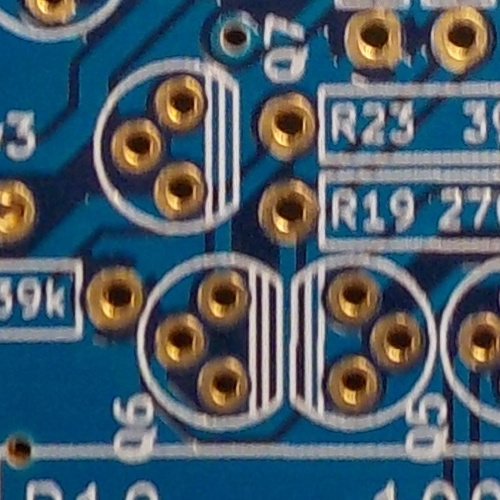
\includegraphics[width={1.50in}]{to92-bar.jpg}\quad
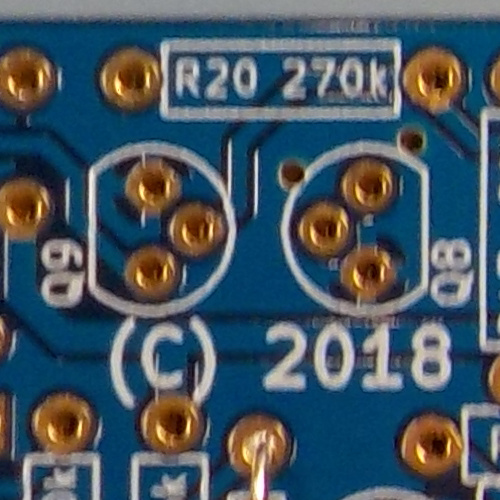
\includegraphics[width={1.50in}]{to92-nobar.jpg}

All TO-92 components in this project are polarized and must be installed in
the correct orientation to work; that orientation is shown by the silkscreen
symbols.  Install each component so that its flat side points in the same
direction as the flat side shown on the silkscreen.  The three legs of the
component must be carefully bent into the same triangular pattern (left and
right forward, middle backward) as the holes on the board, and then the
component pressed into place.  There should be a gap of about three
millimetres between the board and the component body; do not attempt to seat
the component flush on the board because of the risk of breaking off the
legs where they enter the body.

The solder pads for these components are smaller and closer together than
for any other through-hole components in the project, and the components
themselves tend to be relatively heat-sensitive.  Solder them carefully,
avoiding creating any solder bridges between adjacent pads.  Do not use
excessive time and heat trying to get the solder to flow through the board
and fillet on both sides, especially not on pads connected to the ground
plane; two-sided fillets are nice if they happen naturally, but it is good
enough for solder to completely cover the pad on one side.

Install the five 2N5088 NPN transistors Q1, Q2, Q4, Q8, and Q9.  Most of
these act as switches in the input Schmitt trigger and attack flip-flop; Q4
forms part of the output buffer Sziklai pair.

\noindent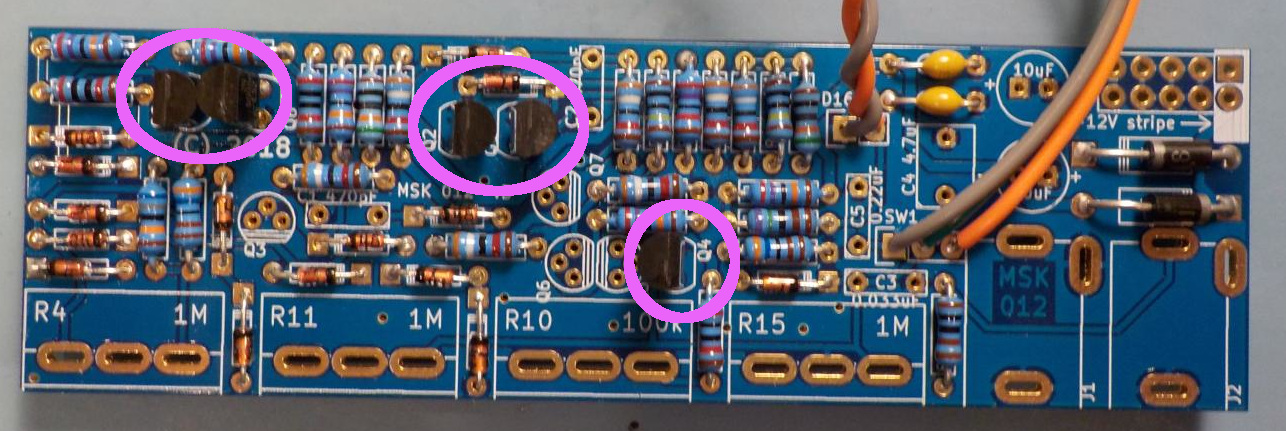
\includegraphics[width=\linewidth]{2n5088.jpg}

Install the four SS8550D or PN200A PNP transistors Q3, Q5, Q6, and Q7.  The
first, Q3, sinks current away from the envelope capacitor during the release
and sustain phases; Q5 forms part of the output buffer Sziklai pair; and Q6
and Q7 act as switches in the output Schmitt trigger.

\noindent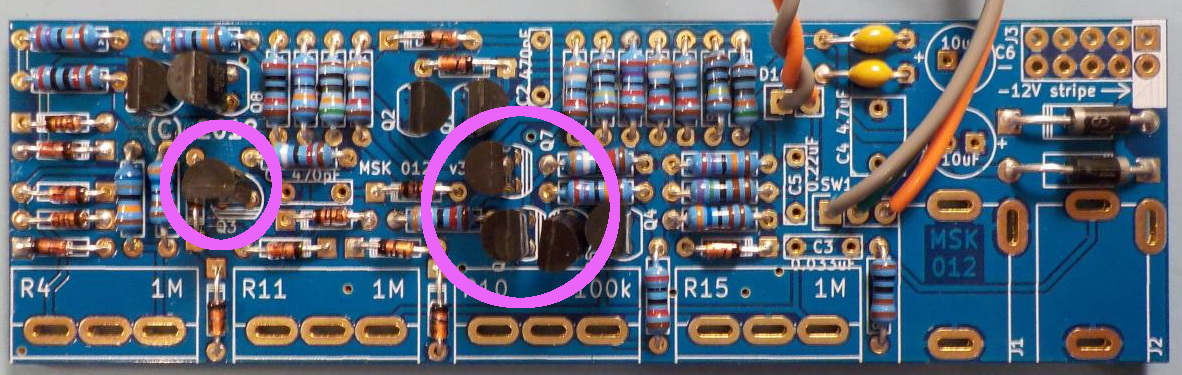
\includegraphics[width=\linewidth]{pn200a.jpg}

\pagebreak

\section{Capacitors}

Install the two 470pF ceramic capacitors C1 and C2.  These capacitors form
pulses from the switching transitions of the input and output Schmitt
triggers.  They are not polarized and may be installed in either direction. 
They will probably be marked ``471,'' which indicates the number of
picofarads using something like the resistor code:  significant digits 4~7
followed by 1 zero, that is, ``470pF.''

\nopagebreak
\noindent\includegraphics[width=\linewidth]{{cap-470p}.jpg}

Install the 0.033$\mu$F film capacitor C3.  This capacitor stores the
envelope voltage in the fastest speed range, also taking a small part in the
other two speed ranges.  It is not polarized and may be installed in either
direction.

\noindent\includegraphics[width=\linewidth]{{cap-0.033u}.jpg}

Install the 0.22$\mu$F film capacitor C5.  This capacitor stores the
envelope voltage in the middle speed range.  It is not polarized and may be
installed in either direction.

\noindent\includegraphics[width=\linewidth]{{cap-0.22u}.jpg}

Install the 4.7$\mu$F film capacitor C4.  This capacitor stores the
envelope voltage in the slow speed range.  It is not polarized and may be
installed in either direction.

\noindent\includegraphics[width=\linewidth]{{cap-4.7u}.jpg}

Install the two 10$\mu$F electrolytic capacitors C6 and C7.  These filter
lower-frequency interference on the power lines.
They are polarized components, and may explode if connected
backwards.  As such, there are multiple clues to help you install them in
the right direction.  The negative leg of each capacitor will be marked in
some way, usually with a printed stripe and minus signs on the plastic
wrapping of the capacitor body.  The negative leg of the capacitor will
usually also be shorter, though that is less reliable than the body
markings.  On the PCB, the positive and negative pads are marked with
positive and negative signs in the silkscreen, and the solder pads
themselves are round for negative and square for positive.

\noindent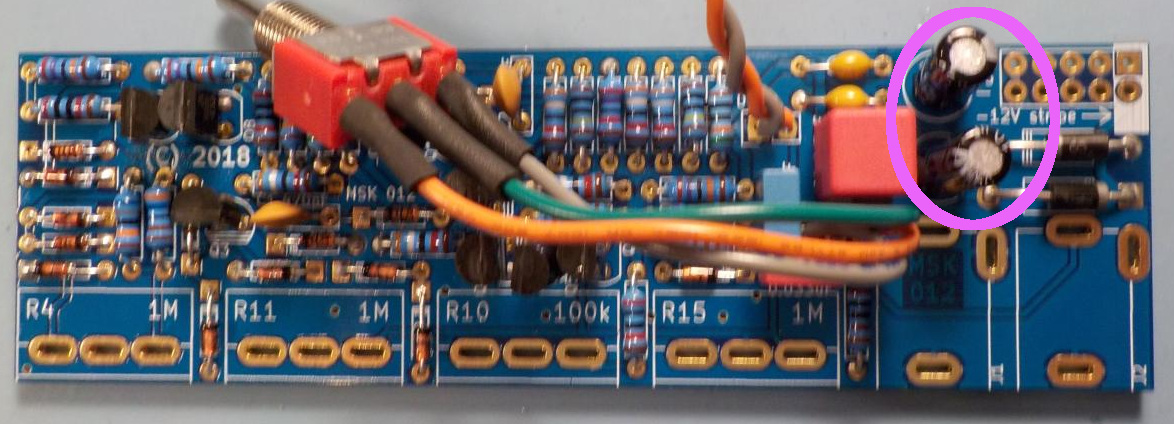
\includegraphics[width=\linewidth]{cap-10u.jpg}

\section{Power header}

Install the 10-pin dual-row Eurorack power header J3.
It is not polarized
in the horizontal plane.  However, if it has shorter legs on one side, then
those are the ones that should go through the PCB (leaving the longer legs
sticking up to mate with the connector on the power cable), and if it has
tin plating on one end of the pins and gold on the other, then the tin side
should be the one soldered through the board.  Secure the header carefully
to the board, possibly with tape, before soldering it.  It is easy to
accidentally solder it at an angle, which is a difficult error to fix and
may cause trouble when you later attach the power cable.

\noindent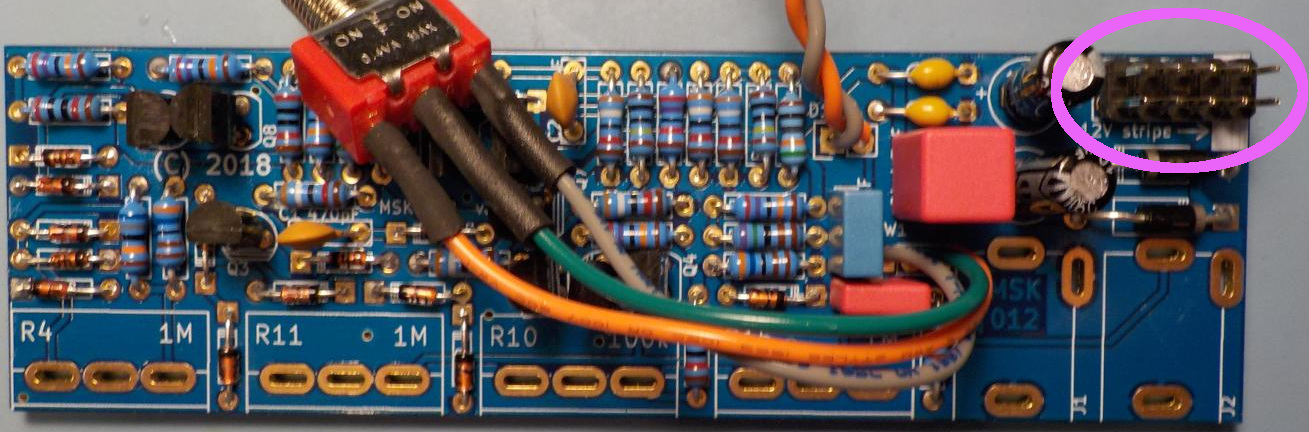
\includegraphics[width=\linewidth]{power.jpg}

Note that Eurorack power connections are polarized even if the connectors
are not.  The cables are usually grey ribbon type with a red stripe along
one side indicating pin 1, which carries $-$12V power.  For most modules
including the MSK~012, the red stripe should be at the \emph{bottom} when
the module is mounted vertically in a case.  On the MSK~012, the correct
location of the $-$12V supply is also marked with the text ``$-$12V
stripe,'' arrows, and a white area on both sides of the PCB silkscreen. 
This module is also protected (by the Schottky diodes you just installed)
from damage in case of a reversed power connection; if you connect the power
backwards and nothing else is wrong, then the module will not power up but
will be fine once you connect the power correctly.  However, many other
modules are not so protected, and it is dangerous to get into the habit of
depending on protection diodes.  Destroying a module by connecting power
backwards is almost a rite of passage for Eurorack users.

\section{Panel components}

Sourcing good-quality panel potentiometers with all the right features for a
given project is difficult, and for the MSK~012, the closest I was able to
come was to find a type with right-angle bent terminals, where the physical
design of the module requires straight PCB terminals.  So, if you are using
the potentiometers supplied in a North Coast kit or close equivalents to
them, your potentiometers will probably resemble the one at left in the
photo, with its terminals bent downward.  Carefully bend the terminals with
pliers so that they lie in roughly the same plane as the fibreglass panel of
the potentiometer, as shown at right in the photo.

\noindent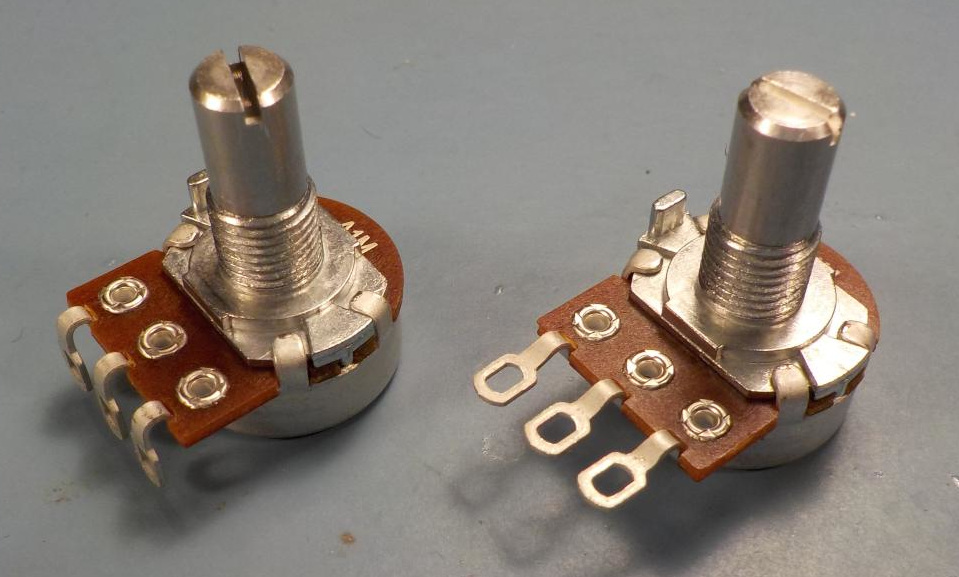
\includegraphics[width=\linewidth]{bend-pots.jpg}

Consult the exploded assembly diagram on page~\pageref{fig:exploded} for
details of how the following parts fit together.

Install the four potentiometers (R4, R10, R11, and R15) in the panel with
their supplied hardware, but only \emph{very loosely} at this point; they
should be just tight enough to keep the anti-rotation tabs in the
corresponding holes, with enough play for subsequent steps to position them
exactly.  Take careful note of which one of these is R10, the 100k$\Omega$
unit; it must go in the hole labelled ``S,'' third from the top end of the
panel.  Snap the LED mounting clip (small black plastic object) into the
panel hole above the words ``NORTH COAST.'' Install the two panel jack
sockets (J1 and J2) in their respective holes.

\noindent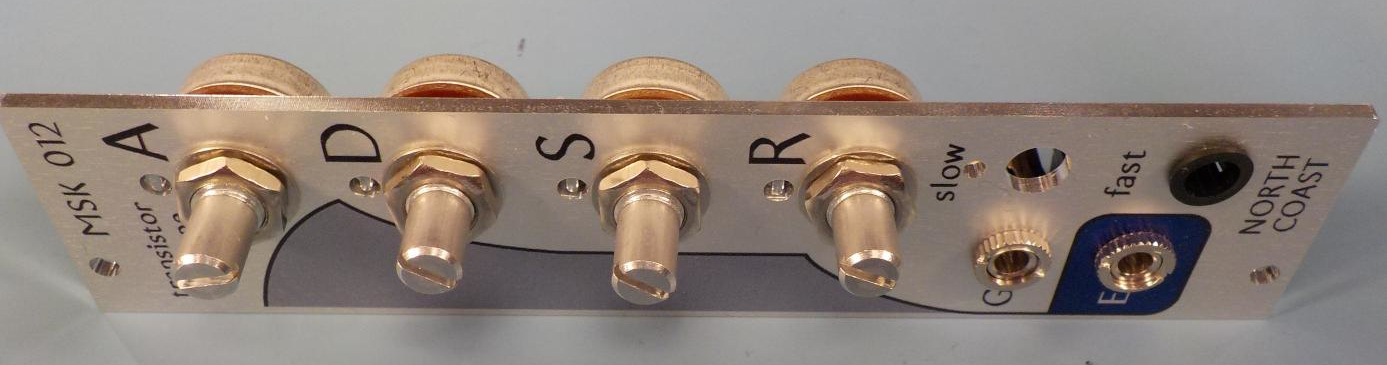
\includegraphics[width=\linewidth]{panel-parts1.jpg}

Fit the PCB onto the protruding legs of the potentiometers and jack sockets. 
It may be necessary to adjust the bends a little to get all legs to fit. 
Try to get the PCB at right angles to the panel as nearly as possible.  Then
tighten the nuts on the potentiometers, and solder all these components.

Push the switch and LED into their corresponding holes in the panel, with
the LED fitting inside its mounting clip.  The keyway on the switch must
face toward the top end of the panel so that the tabs on the anti-rotation
ring can fit into the switch keyway and the small panel hole.  The switch
will probably come with two nuts.  When tightening them, do not overtighten;
overenthusiastic use of a wrench can pull the bushing right off of the
switch, destroying it.

\noindent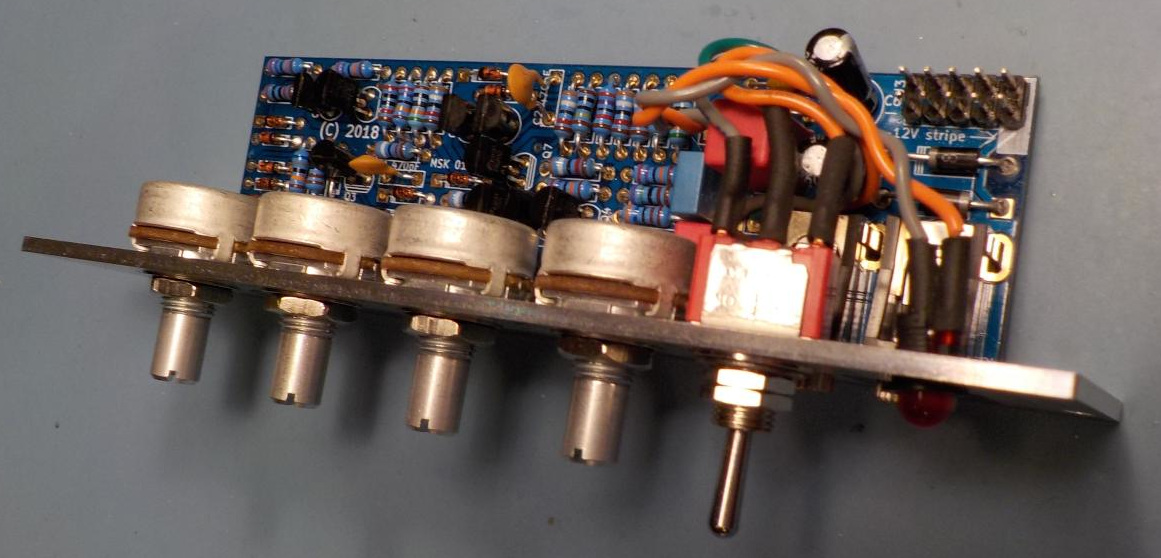
\includegraphics[width=\linewidth]{panel-parts2.jpg}

Attach the knobs to the potentiometers.  Twist each shaft to its limits in
each direction to ascertain how the slot in the shaft corresponds to where
you want the knob pointer, then slide the knob onto the shaft in the correct
orientation and tighten the setscrew with a small flat screwdriver.  Do not
fasten the knobs pushed all the way down onto the shafts, or they will rub
against the bushings and be hard to turn; instead, back them off about a
millimetre from the bottom.

There is a rectangular white area on the back of the board
reserved for adding a serial number, signature, quality control marking, or
similar.  Use a fine-tipped permanent marker to write whatever you want
there.

Your module is complete.

\noindent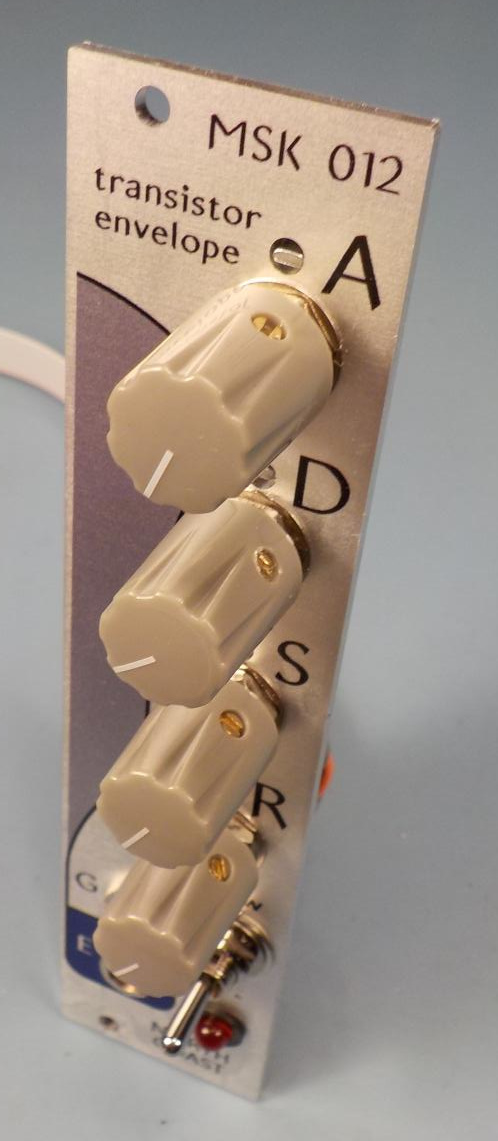
\includegraphics[width=\linewidth]{finished-module.jpg}
